\documentclass[12pt,a4paper]{article}
\usepackage[top=2.5cm,bottom=2.5cm,left=2.5cm,right=2.5cm,headheight=15pt]{geometry}
\usepackage{amsmath,amssymb}
\usepackage{tikz}
\usetikzlibrary{shapes,arrows,arrows.meta,positioning,calc,backgrounds,fit}
\usepackage{booktabs,array,longtable,tabularx,multirow}
\usepackage{xcolor}
\usepackage{enumitem}
\usepackage{fancyhdr}
\usepackage{titlesec}
\usepackage{mdframed}
\usepackage{tcolorbox}
\tcbuselibrary{skins,breakable}
\usepackage{hyperref}

%% ---- Colors ----
\definecolor{ruleblue}{RGB}{0,82,165}
\definecolor{lightblue}{RGB}{220,235,255}
\definecolor{darkteal}{RGB}{0,105,92}
\definecolor{lightteal}{RGB}{200,230,225}
\definecolor{darkorange}{RGB}{180,70,0}
\definecolor{lightorange}{RGB}{255,235,210}
\definecolor{darkgreen}{RGB}{20,110,20}
\definecolor{lightgreen}{RGB}{200,240,205}
\definecolor{darkred}{RGB}{150,20,20}
\definecolor{lightred}{RGB}{255,210,210}
\definecolor{lightgray}{RGB}{242,242,242}
\definecolor{dpurple}{RGB}{90,0,140}
\definecolor{lpurple}{RGB}{235,215,255}

%% ---- tcolorbox styles ----
\newtcolorbox{defbox}[1]{enhanced,breakable,
  colback=lightblue,colframe=ruleblue,arc=4pt,
  title={\textbf{#1}},fonttitle=\bfseries\color{white},
  attach boxed title to top left={yshift=-2mm,xshift=4mm},
  boxed title style={colback=ruleblue,arc=3pt}}

\newtcolorbox{exambox}[1]{enhanced,breakable,
  colback=lightorange,colframe=darkorange,arc=4pt,
  title={\textbf{#1}},fonttitle=\bfseries\color{white},
  attach boxed title to top left={yshift=-2mm,xshift=4mm},
  boxed title style={colback=darkorange,arc=3pt}}

\newtcolorbox{keybox}[1]{enhanced,breakable,
  colback=lightgreen,colframe=darkgreen,arc=4pt,
  title={\textbf{#1}},fonttitle=\bfseries\color{white},
  attach boxed title to top left={yshift=-2mm,xshift=4mm},
  boxed title style={colback=darkgreen,arc=3pt}}

\newtcolorbox{algobox}[1]{enhanced,breakable,
  colback=lightgray,colframe=gray!60,arc=4pt,
  title={\textbf{#1}},fonttitle=\bfseries,
  attach boxed title to top left={yshift=-2mm,xshift=4mm},
  boxed title style={colback=gray!60,arc=3pt}}

%% ---- Page style ----
\pagestyle{fancy}\fancyhf{}
\lhead{\color{ruleblue}\textbf{Rule-Based Systems --- CSE 713 AI}}
\rhead{\color{ruleblue}Exam: 10 Jun 2026}
\cfoot{--- \thepage\ ---}
\renewcommand{\headrulewidth}{0.4pt}

%% ---- Section styles ----
\titleformat{\section}{\Large\bfseries\color{ruleblue}}{\thesection.}{0.5em}{}[\color{ruleblue}\titlerule]
\titleformat{\subsection}{\large\bfseries\color{darkteal}}{\thesubsection.}{0.5em}{}
\titleformat{\subsubsection}{\normalsize\bfseries\color{darkorange}}{\thesubsubsection.}{0.5em}{}

%% ---- TikZ node styles ----
\tikzset{
  rbs/.style={rectangle,rounded corners=5pt,draw=#1!80,fill=#1!15,
              text centered,font=\small\bfseries},
  factN/.style={ellipse,draw=darkorange,fill=lightorange,
                minimum width=1.1cm,minimum height=0.6cm,font=\small\bfseries},
  derivN/.style={ellipse,draw=ruleblue,fill=lightblue,
                 minimum width=1.1cm,minimum height=0.6cm,font=\small\bfseries},
  goalN/.style={ellipse,draw=darkgreen,fill=lightgreen,
                minimum width=1.1cm,minimum height=0.6cm,font=\small\bfseries},
  bcG/.style={rectangle,rounded corners=3pt,draw=ruleblue,fill=lightblue,
              minimum width=1.3cm,minimum height=0.55cm,font=\small\bfseries},
  bcP/.style={ellipse,draw=darkgreen,fill=lightgreen,
              minimum width=1.0cm,minimum height=0.5cm,font=\small\bfseries},
  bcF/.style={ellipse,draw=darkred,fill=lightred,
              minimum width=1.0cm,minimum height=0.5cm,font=\small,text=darkred},
  arr/.style={-{Stealth[length=5pt]},thick},
  darr/.style={-{Stealth[length=4pt]},thick,dashed,gray},
}

\hypersetup{colorlinks=true,linkcolor=ruleblue,urlcolor=darkteal,
  pdftitle={Rule-Based Systems CSE713}}

\begin{document}

%% ===================== TITLE =====================
\begin{center}
{\Huge\bfseries\color{ruleblue}Rule-Based Systems}\\[0.4cm]
{\large Complete Study Guide with Past Paper Solutions (2020--2024)}\\[0.2cm]
{\normalsize CSE 713 --- Artificial Intelligence \quad|\quad University of Chittagong \quad|\quad Exam: 10 Jun 2026}\\[0.2cm]
\rule{14cm}{0.5pt}
\end{center}

\begin{tcolorbox}[colback=lightblue,colframe=ruleblue]
\textbf{Topics:} RBS Introduction $\bullet$ Architecture (TikZ) $\bullet$ Conflict Resolution $\bullet$
Forward Chaining $\bullet$ Backward Chaining $\bullet$ FC vs BC $\bullet$
Canonical Exam Problem (R1--R5, prove G) $\bullet$ Expert Systems $\bullet$ Frames
\end{tcolorbox}

\tableofcontents\newpage

%%==============================================
\section{Introduction to Rule-Based Systems}
%%==============================================

\begin{defbox}{Definition}
A \textbf{Rule-Based System (RBS)} is a system whose knowledge base (KB) is represented as a
collection of \textbf{IF--THEN rules} (the rule base) and \textbf{facts} (the fact base), together with
an \textbf{inference engine} that controls how rules are applied to facts to derive new knowledge.
\[
\text{RBS} = \text{Rule Base} + \text{Fact Base} + \text{Inference Engine}
\]
\end{defbox}

\subsection{Knowledge Representation: Rules and Facts}

In logic, knowledge is represented in a \textit{declarative and static} manner.
Well-formed formulas (wffs) in propositional logic or FOL are divided into two categories:

\begin{itemize}[itemsep=4pt]
  \item \textbf{Rules} --- assertions in \textit{implication form}:
        \texttt{IF}\,\(\langle\text{condition}\rangle\)\,\texttt{THEN}\,\(\langle\text{action}\rangle\).
        A rule tells the system \emph{what to do or derive} when conditions are met.
  \item \textbf{Facts} --- domain-specific assertions that are currently known to be true.
        Facts reside in the \textbf{Working Memory (WM)}.
\end{itemize}

\textbf{Logic vs.\ RBS:} In logic, rules say what is \textit{TRUE} given conditions.
In RBS, rules say what to \textit{DO} (e.g., add a new fact) given conditions.
A special interpreter (the inference engine) controls when and which rules are invoked.

\subsection{Structure of a Rule}

Every rule takes the form:
\[
\underbrace{\texttt{IF}\;\;P_1\;\texttt{AND}\;P_2\;\texttt{AND}\;\cdots\;\texttt{AND}\;P_n}_{\text{Antecedent / LHS}}
\;\;\texttt{THEN}\;\;
\underbrace{Q}_{\text{Consequent / RHS}}
\]

Key points:
\begin{itemize}
  \item If the antecedent is \textbf{NULL}, the rule becomes an unconditional \textbf{fact}.
  \item Rules are normally represented as \textbf{Horn clauses} --- clauses with
        \emph{at most one positive literal}: \(\neg P_1\vee\cdots\vee\neg P_n\vee Q\),
        equivalent to \(P_1\wedge\cdots\wedge P_n\Rightarrow Q\).
\end{itemize}

\subsection{Triggered vs.\ Fired Rules}

\begin{itemize}
  \item A rule is \textbf{triggered} when \emph{all} its antecedent conditions evaluate to TRUE in WM.
        All currently triggered rules form the \textbf{conflict set}.
  \item A rule is \textbf{fired} when it is \emph{selected} from the conflict set by the conflict-resolution
        strategy and its consequent is executed (typically: add a new fact to WM).
\end{itemize}

%%==============================================
\section{Architecture of a Rule-Based System}
%%==============================================

\begin{exambox}{Past Paper (Every Year 2020--2024)}
``Draw the architecture of a rule-based system.''\\
2024~Q6c [5.5\,m], 2023~Q6c [6\,m], 2022~B-3, 2021~Q5c [5.75\,m], 2020~Q5c [5.75\,m]
\end{exambox}

\subsection{Five Major Components}

\begin{enumerate}[itemsep=5pt]
  \item \textbf{Rule Base} --- the static set of IF--THEN rules encoding expert knowledge.
  \item \textbf{Fact Base (Database of Facts)} --- the initial known facts about the problem.
        Loaded into Working Memory at startup.
  \item \textbf{Working Memory (WM)} --- a \emph{dynamic} store of all currently known facts
        (initial + derived). Updated continuously as rules fire.
  \item \textbf{Inference Engine} --- the ``brain''. Reads rules from the Rule Base, matches them
        against WM, selects one rule to fire (conflict resolution), updates WM.
        Operates in the \textbf{Match--Resolve--Act cycle}.
  \item \textbf{User Interface / Explanation Facility} --- enables user interaction and answers
        ``Why?'' (why is this question asked) and ``How?'' (how was this conclusion reached).
\end{enumerate}

\subsection{Architecture Diagram}

\begin{center}
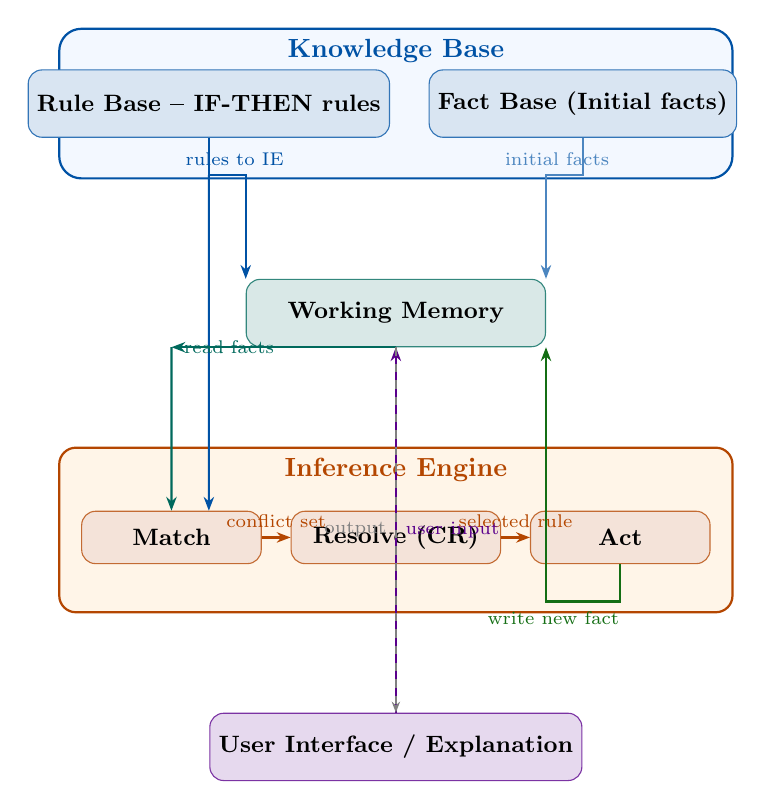
\begin{tikzpicture}[scale=0.95,transform shape]

%% ---- Knowledge Base box ----
\draw[rounded corners=8pt,draw=ruleblue,fill=lightblue!35,thick]
  (-4.5,0.6) rectangle (4.5,-1.4);
\node[font=\bfseries\color{ruleblue}] at (0,0.3) {Knowledge Base};

%% Rule Base
\node[rbs=ruleblue,minimum width=3.8cm,minimum height=0.9cm] (rb) at (-2.5,-0.4)
  {Rule Base -- IF-THEN rules};

%% Fact Base
\node[rbs=ruleblue,minimum width=3.8cm,minimum height=0.9cm] (fb) at (2.5,-0.4)
  {Fact Base (Initial facts)};

%% Working Memory
\node[rbs=darkteal,minimum width=4.0cm,minimum height=0.9cm] (wm) at (0,-3.2)
  {Working Memory};

%% Inference Engine (outer)
\draw[rounded corners=6pt,draw=darkorange,fill=lightorange!50,thick]
  (-4.5,-5.0) rectangle (4.5,-7.2);
\node[font=\bfseries\color{darkorange}] at (0,-5.3) {Inference Engine};

\node[rbs=darkorange,minimum width=2.4cm,minimum height=0.7cm] (match)  at (-3.0,-6.2) {Match};
\node[rbs=darkorange,minimum width=2.8cm,minimum height=0.7cm] (resolve) at (0,-6.2) {Resolve (CR)};
\node[rbs=darkorange,minimum width=2.4cm,minimum height=0.7cm] (act)    at (3.0,-6.2) {Act};

%% Explanation Facility
\node[rbs=dpurple,minimum width=4.0cm,minimum height=0.9cm] (ef) at (0,-9.0)
  {User Interface / Explanation};

%% Arrows from KB to WM/IE
\draw[arr,ruleblue] (rb.south) -- ++(0,-0.5) -| (wm.north west)
  node[pos=0.35,above,font=\scriptsize]{rules to IE};
\draw[arr,ruleblue!70] (fb.south) -- ++(0,-0.5) -| (wm.north east)
  node[pos=0.35,above,font=\scriptsize]{initial facts};
\draw[arr,ruleblue] (rb.south) ++(0,-0.5) coordinate(rbmid)
  -- (rbmid|-match.north);

%% WM ↔ Inference Engine
\draw[arr,darkteal] (wm.south) -- node[left,font=\scriptsize]{read facts} (match.north|-wm.south) coordinate(wmS);
\draw[arr,darkteal] (wmS) -- (match.north);
\draw[arr,darkgreen] (act.south) -- ++(0,-0.5) -| (wm.south east)
  node[pos=0.45,below,font=\scriptsize]{write new fact};

%% Match→Resolve→Act
\draw[arr,darkorange] (match.east) -- node[above,font=\scriptsize]{conflict set} (resolve.west);
\draw[arr,darkorange] (resolve.east) -- node[above,font=\scriptsize]{selected rule} (act.west);

%% IE ↔ EF
\draw[arr,dpurple] (ef.north) -- node[right,font=\scriptsize]{user input} (wm.south);
\draw[darr] (wm.south) -- node[left,font=\scriptsize]{output} (ef.north);

\end{tikzpicture}
\end{center}

\subsection{The Match--Resolve--Act Cycle}

\begin{enumerate}[itemsep=5pt]
  \item \textbf{Match} --- Compare every rule's antecedents against WM.
        All fully satisfied rules form the \textbf{conflict set}.
  \item \textbf{Resolve} --- Select one rule from the conflict set using a
        \textbf{conflict-resolution strategy}.
  \item \textbf{Act} --- Execute the selected rule's action: add, modify, or delete facts in WM.
\end{enumerate}

Repeat until: (a) no rules are applicable (\emph{quiescence}), or (b) the goal fact is in WM.

%%==============================================
\section{Conflict Resolution}
%%==============================================

\begin{defbox}{Definition}
\textbf{Conflict resolution} is the process of deciding \emph{which rule} from the conflict set
(all currently triggered rules) should be \emph{fired} when multiple rules are simultaneously applicable.
\end{defbox}

\begin{exambox}{Past Paper (Every Year 2020--2024)}
``What is conflict resolution? Discuss any two approaches.''\\
2024~Q6b [1.5\,m], 2023~Q6b [1\,m], 2022~B-3a [2\,m], 2021~Q5b [1.5\,m], 2020~Q5b [1.5\,m]
\end{exambox}

\textbf{Why needed:} At any cycle, multiple rules may be triggered.
Firing different rules can lead to different conclusions or efficiency.
Note: 90\% of RBS computing time is spent in the match phase, so efficient resolution matters.

\subsection{Conflict Resolution Strategies}

\begin{center}
\renewcommand{\arraystretch}{1.45}
\begin{tabular}{>{\bfseries}p{4.0cm} p{9.5cm}}
\toprule
Strategy & Description \\
\midrule
1.\ Rule Ordering (FCFS) &
  Fire the rule that appears \emph{first} in the rule base.
  Simple; the knowledge engineer orders rules by priority. \\

2.\ Specificity Ordering &
  Fire the rule with the \emph{most specific} conditions (most antecedents).
  More specific rules are assumed more relevant to the current situation. \\

3.\ Recency &
  Fire the rule whose antecedents match the \emph{most recently added} facts in WM.
  Keeps reasoning focused on new information. \\

4.\ Fire All &
  Fire \emph{all} triggered rules in one cycle.
  Faster convergence but risks inconsistency. \\

5.\ Heuristic Measure &
  Fire the rule estimated to bring WM \emph{closest to the goal}
  (minimum distance heuristic). \\

6.\ \textbf{Refractoriness} &
  A rule fired for a given set of facts will \emph{not be fired again for the same facts}.
  Prevents infinite loops. Not a selection strategy, but a prevention mechanism. \\

7.\ Meta-Rules &
  \emph{Rules about rules} embedded in the inference engine specifying which rules
  apply under which high-level conditions. \\
\bottomrule
\end{tabular}
\end{center}

\begin{keybox}{Exam Answer Template}
Define conflict resolution (1 sentence).
Then explain two strategies in detail.
\textbf{Best pair}: Rule Ordering (FCFS) + Specificity Ordering.
Mention Refractoriness as a bonus point.
\end{keybox}

%%==============================================
\section{Forward Chaining (Data-Driven Reasoning)}
%%==============================================

\begin{defbox}{Definition}
\textbf{Forward chaining (FC)} is a \emph{data-driven} (bottom-up) inference strategy
where reasoning starts from the \textbf{known facts} and applies rules to derive new facts,
progressively working \emph{toward} the goal.
Also called: data-driven search, antecedent-driven, bottom-up reasoning.
\end{defbox}

\subsection{Mechanism}

Facts are held in \textbf{Working Memory (WM)}.
Condition-action rules represent actions to take (add/delete facts from WM) when conditions are met.
The inference engine runs the \emph{Recognize--Act cycle}:

\begin{algobox}{Forward Chaining Algorithm}
\begin{verbatim}
ForwardChaining(Rules R, Initial Facts F, Goal G):
  WM := F
  WHILE G not in WM:
    conflict_set := { r in R | all antecedents of r satisfied in WM
                              AND r not yet fired for these facts }
    IF conflict_set = empty  THEN RETURN FAILURE
    r* := ConflictResolution(conflict_set)
    WM := WM UNION { consequent of r* }
    MARK r* as fired (refractoriness)
  RETURN SUCCESS
\end{verbatim}
\end{algobox}

\subsection{Backtracking in FC}

FC may reach a \textbf{dead end}: rules fired but goal unreachable and no new rules fire.
Two backtracking strategies:
\begin{itemize}
  \item \textbf{Chronological}: Undo the most recent decision; try the next alternative.
  \item \textbf{Intelligent (dependency-directed)}: Identify exactly which earlier decision
        caused the failure; undo only that. More efficient.
\end{itemize}

\subsection{When to Use Forward Chaining}

\begin{itemize}
  \item When \textbf{all or most data is already known} (rich initial WM).
  \item When the \textbf{goal is not specific} --- you want to see what can be derived.
  \item When there are \textbf{many possible goals} and you want to find any one.
  \item Applications: monitoring systems, planning, CLIPS-based expert systems.
\end{itemize}

%%==============================================
\section{Backward Chaining (Goal-Directed Reasoning)}
%%==============================================

\begin{defbox}{Definition}
\textbf{Backward chaining (BC)} is a \emph{goal-directed} (top-down) inference strategy
where reasoning starts from the \textbf{goal (hypothesis)} and works backward to find
supporting facts. It asks: ``What must be true for this goal to hold?''
Also called: goal-driven, consequent-driven, top-down reasoning.
\end{defbox}

\subsection{Mechanism}

Start with goal $G$.
Find a rule $R$ whose consequent matches $G$.
Treat $R$'s antecedents as new sub-goals to prove recursively.
Each sub-goal is either in the initial facts (proved) or requires another rule.
Backtrack if no rule can prove a sub-goal.

\begin{algobox}{Backward Chaining Algorithm (Recursive)}
\begin{verbatim}
BackwardChaining(Goal G, Facts F, Rules R):
  IF G in F:
    RETURN TRUE          -- G is a known fact
  FOR each rule r: (C1 AND C2 AND ... Cn => G) in R:
    all_proved := TRUE
    FOR each Ci in {C1,...,Cn}:
      IF NOT BackwardChaining(Ci, F, R):
        all_proved := FALSE
        BREAK            -- this rule branch fails; try next
    IF all_proved:
      RETURN TRUE        -- G proved via rule r
  RETURN FALSE           -- no rule could prove G
\end{verbatim}
\end{algobox}

\textbf{Why more focused than FC:}
FC fires any applicable rule, possibly deriving many irrelevant conclusions.
BC only explores rules relevant to the current goal --- no wasted effort.
\textbf{PROLOG} uses BC as its built-in reasoning mechanism.

\subsection{When to Use Backward Chaining}

\begin{itemize}
  \item When the \textbf{goal is specific and well-known} upfront.
  \item When there are \textbf{few competing hypotheses} to test.
  \item When \textbf{data acquisition is costly} (BC only asks for data it needs).
  \item Applications: medical diagnosis (MYCIN), PROLOG queries.
\end{itemize}

%%==============================================
\section{Forward Chaining vs.\ Backward Chaining}
%%==============================================

\begin{exambox}{Past Paper (Every Year 2020--2024)}
``Define forward and backward chaining. What factors determine whether to use FC or BC?''\\
2024~Q6a [2\,m], 2023~Q6a [2\,m], 2022~B-3b [1.5\,m], 2021~Q5a [1.5\,m], 2020~Q5a [1.5\,m]
\end{exambox}

\begin{center}
\renewcommand{\arraystretch}{1.45}
\begin{tabular}{>{\bfseries}p{3.6cm} p{4.9cm} p{4.9cm}}
\toprule
Property & Forward Chaining & Backward Chaining \\
\midrule
Direction          & Facts $\rightarrow$ Goal       & Goal $\rightarrow$ Facts \\
Reasoning style    & Data-driven, bottom-up         & Goal-driven, top-down \\
Starting point     & Known facts in WM              & Hypothesis / Goal \\
Approach           & Derive all possible facts      & Reduce goal to sub-goals \\
Risk               & Irrelevant conclusions         & Dead-end branches \\
Best when          & Much data; goal not specific   & Specific goal; sparse data \\
Data acquisition   & All data gathered upfront      & Only fetches needed data \\
Analogy            & Scientist making observations  & Doctor testing a diagnosis \\
Used in            & CLIPS, monitoring, planning    & PROLOG, MYCIN, diagnosis \\
\bottomrule
\end{tabular}
\end{center}

\subsection{Factors for Choosing FC vs.\ BC}

\begin{enumerate}[itemsep=6pt]
  \item \textbf{Nature of the initial data:}
        Many known facts $\Rightarrow$ \textbf{FC}.
        Sparse data, specific hypothesis $\Rightarrow$ \textbf{BC}.

  \item \textbf{Nature of the goal:}
        Many possible goals (find any) $\Rightarrow$ \textbf{FC}.
        Single specific goal to confirm/deny $\Rightarrow$ \textbf{BC}.

  \item \textbf{Branching factor:}
        One fact triggers many rules (high forward branching) $\Rightarrow$ \textbf{BC} more efficient.
        One goal has many possible supporting rules (high backward branching) $\Rightarrow$ \textbf{FC} may be better.

  \item \textbf{Cost of data acquisition:}
        Data freely available $\Rightarrow$ \textbf{FC}.
        Data must be acquired (user asked, tests run) $\Rightarrow$ \textbf{BC} (only requests what is needed).
\end{enumerate}

%%==============================================
\section{Canonical Exam Problem: Prove Goal G}
%%==============================================

\begin{exambox}{Problem Statement --- 2024 Q6c, 2023 Q6c, 2022 B-3c, 2021 Q5c, 2020 Q5c}
\textbf{Rule Base:}
\begin{align*}
  \text{R1:} & \quad \text{IF } A \wedge C \text{ THEN } E \\
  \text{R2:} & \quad \text{IF } C \wedge D \text{ THEN } F \\
  \text{R3:} & \quad \text{IF } B \wedge E \text{ THEN } F \\
  \text{R4:} & \quad \text{IF } B \text{ THEN } C \\
  \text{R5:} & \quad \text{IF } F \text{ THEN } G
\end{align*}
\textbf{Initial facts:} $A$ and $B$ (both true). \quad \textbf{Goal:} Prove $G$.\\
Show rule firing sequence and draw the search tree for both FC and BC.
\end{exambox}

\subsection{Part (a): Forward Chaining Solution}

\textbf{Strategy:} WM $=\{A,B\}$. Each cycle: find triggered rules, apply conflict resolution
(rule ordering: fire lowest-numbered applicable rule), fire it, add conclusion to WM.
Repeat until $G$ appears.

\subsubsection{Step-by-Step FC Trace}

\begin{center}
\renewcommand{\arraystretch}{1.55}
\begin{longtable}{c p{3.6cm} p{3.8cm} c p{3.5cm}}
\toprule
\textbf{Cycle} & \textbf{Working Memory} & \textbf{Rules Checked} &
\textbf{Conflict Set} & \textbf{Action} \\
\midrule
\endfirsthead
\toprule
Cycle & Working Memory & Rules Checked & Conflict Set & Action \\
\midrule
\endhead
0 & $\{A,\,B\}$ & --- & --- & Initialization \\
\midrule
1 & $\{A,\,B\}$ &
  R1: A$\checkmark$ C?\texttimes{} $\Rightarrow$ No\newline
  R2: C?\texttimes{} $\Rightarrow$ No\newline
  R3: B$\checkmark$ E?\texttimes{} $\Rightarrow$ No\newline
  \textbf{R4: B$\checkmark$ $\Rightarrow$ Yes}\newline
  R5: F?\texttimes{} $\Rightarrow$ No
  & \{R4\} & \textbf{Fire R4:} add $C$ to WM \\
\midrule
2 & $\{A,\,B,\,C\}$ &
  \textbf{R1: A$\checkmark$ C$\checkmark$ $\Rightarrow$ Yes}\newline
  R2: C$\checkmark$ D?\texttimes{} $\Rightarrow$ No\newline
  R3: B$\checkmark$ E?\texttimes{} $\Rightarrow$ No\newline
  R4: \textit{fired}\newline
  R5: F?\texttimes{} $\Rightarrow$ No
  & \{R1\} & \textbf{Fire R1:} add $E$ to WM \\
\midrule
3 & $\{A,\,B,\,C,\,E\}$ &
  R1: \textit{fired}\newline
  R2: D?\texttimes{} $\Rightarrow$ No\newline
  \textbf{R3: B$\checkmark$ E$\checkmark$ $\Rightarrow$ Yes}\newline
  R4: \textit{fired}\newline
  R5: F?\texttimes{} $\Rightarrow$ No
  & \{R3\} & \textbf{Fire R3:} add $F$ to WM \\
\midrule
4 & $\{A,\,B,\,C,\,E,\,F\}$ &
  \textbf{R5: F$\checkmark$ $\Rightarrow$ Yes}
  & \{R5\} & \textbf{Fire R5:} add $G$ to WM \\
\midrule
5 & $\{A,\,B,\,C,\,E,\,F,\,\mathbf{G}\}$ & --- & --- & \textbf{GOAL REACHED!} \\
\bottomrule
\end{longtable}
\end{center}

\begin{keybox}{FC Result}
\textbf{Rule firing sequence: R4 $\to$ R1 $\to$ R3 $\to$ R5}\\[3pt]
WM progression:\;
$\{A,B\} \to \{A,B,C\} \to \{A,B,C,E\} \to \{A,B,C,E,F\} \to \{A,B,C,E,F,\mathbf{G}\}$
\end{keybox}

\subsubsection{Forward Chaining Tree (Truth Propagation Diagram)}

Each node is a fact; arrows show which rule derived it and from which antecedents.
Orange nodes = initial facts. Blue nodes = derived facts. Green node = goal.

\begin{center}
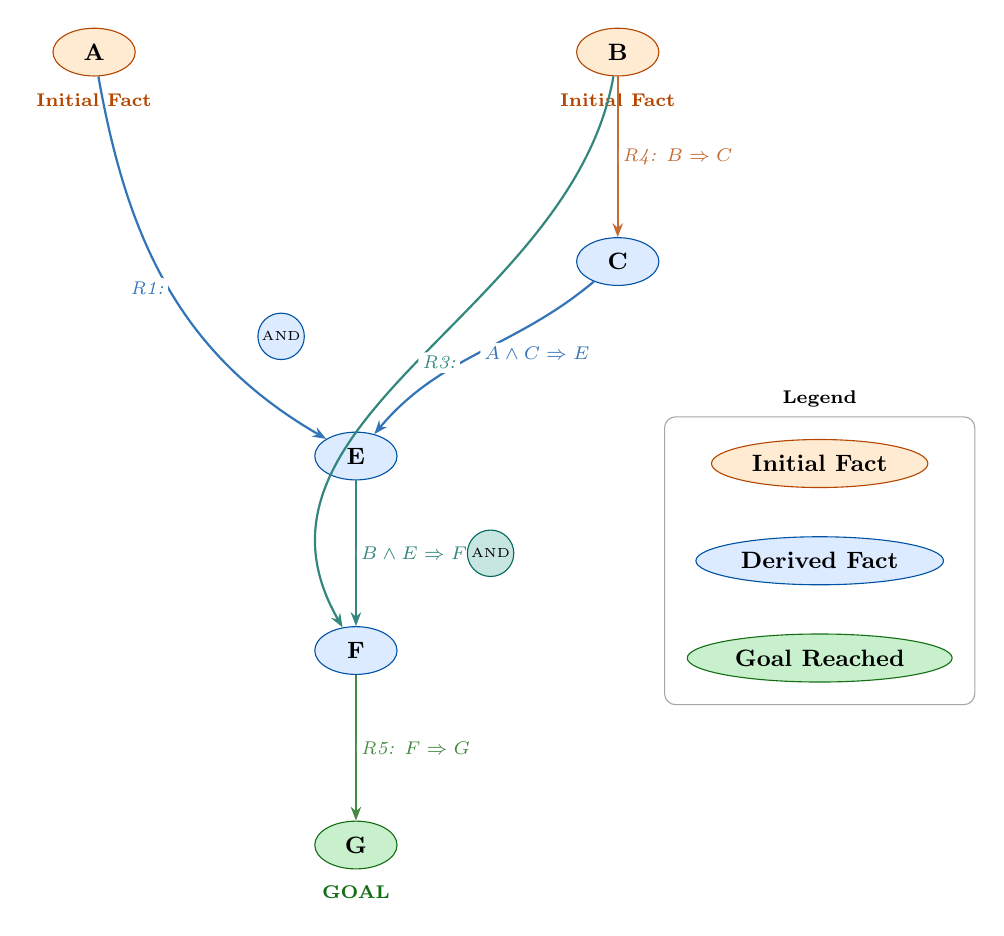
\begin{tikzpicture}[scale=0.95,transform shape,node distance=1.6cm and 2.4cm]

%% Initial facts
\node[factN] (A) at (-3.5,0) {A};
\node[factN] (B) at (3.5,0)  {B};
\node[font=\scriptsize\bfseries\color{darkorange},below=0.1cm of A] {Initial Fact};
\node[font=\scriptsize\bfseries\color{darkorange},below=0.1cm of B] {Initial Fact};

%% Derived C (via R4 from B)
\node[derivN] (C) at (3.5,-2.8) {C};

%% Derived E (via R1 from A and C)
\node[derivN] (E) at (0,-5.4) {E};

%% Derived F (via R3 from B and E)
\node[derivN] (F) at (0,-8.0) {F};

%% Goal G (via R5 from F)
\node[goalN] (G) at (0,-10.6) {\textbf{G}};
\node[font=\scriptsize\bfseries\color{darkgreen},below=0.1cm of G] {GOAL};

%% Rule labels box style
\tikzset{rl/.style={font=\scriptsize\itshape,fill=white,inner sep=1.5pt,rounded corners=2pt}}

%% B → C via R4
\draw[arr,darkorange!80] (B) -- node[right,rl]{R4: $B \Rightarrow C$} (C);

%% A,C → E via R1
\draw[arr,ruleblue!80] (A) to[out=280,in=150]
  node[left,rl]{R1:} (E);
\draw[arr,ruleblue!80] (C) to[out=220,in=50]
  node[right,rl]{$A\wedge C\Rightarrow E$} (E);

%% AND indicator for R1
\node[circle,draw=ruleblue,fill=lightblue,font=\tiny,inner sep=1pt] at (-1.0,-3.8) {AND};

%% B,E → F via R3
\draw[arr,darkteal!80] (B) to[out=260,in=120]
  node[right,rl]{R3:} (F);
\draw[arr,darkteal!80] (E) --
  node[right,rl]{$B\wedge E\Rightarrow F$} (F);

%% AND indicator for R3
\node[circle,draw=darkteal,fill=lightteal,font=\tiny,inner sep=1pt] at (1.8,-6.7) {AND};

%% F → G via R5
\draw[arr,darkgreen!80] (F) --
  node[right,rl]{R5: $F\Rightarrow G$} (G);

%% Legend
\begin{scope}[shift={(6.2,-5.5)}]
\node[factN,minimum width=2.8cm] (l1) at (0,0)   {Initial Fact};
\node[derivN,minimum width=2.8cm] (l2) at (0,-1.3){Derived Fact};
\node[goalN,minimum width=2.8cm] (l3) at (0,-2.6) {Goal Reached};
\node[draw=gray!70,rounded corners=4pt,
      fit=(l1)(l2)(l3),inner sep=8pt,
      label={[font=\scriptsize\bfseries]above:Legend}] {};
\end{scope}

\end{tikzpicture}
\end{center}

\subsection{Part (b): Backward Chaining Solution}

\textbf{Strategy:} Start with goal $G$.
Find rules whose consequent is $G$, treat antecedents as new sub-goals.
Prove each sub-goal recursively.
Backtrack on failure.

\subsubsection{Step-by-Step BC Trace}

\begin{center}
\renewcommand{\arraystretch}{1.55}
\begin{longtable}{c p{2.0cm} p{2.2cm} p{9.2cm}}
\toprule
\textbf{Step} & \textbf{Current Goal} & \textbf{In \{A,B\}?} & \textbf{Action} \\
\midrule
\endfirsthead
\toprule
Step & Goal & In \{A,B\}? & Action \\ \midrule
\endhead
1  & G & No  & Rule with G as consequent: R5 ($F\Rightarrow G$). New sub-goal: \textbf{F} \\
2  & F & No  & Rules with F: R2 ($C\wedge D\Rightarrow F$), R3 ($B\wedge E\Rightarrow F$). Try R2 first. Sub-goals: \textbf{C, D} \\
3  & C & No  & Rule with C: R4 ($B\Rightarrow C$). Sub-goal: \textbf{B} \\
4  & B & \textbf{Yes \checkmark} & B is an initial fact. \textbf{C proved via R4.} \\
5  & D & No  & \textbf{No rule concludes D. D not in facts.}
               \textcolor{darkred}{\textbf{FAIL on D}} $\Rightarrow$ backtrack to Step 2. \\
6  & F & Retry & R2 failed. Try \textbf{R3} ($B\wedge E\Rightarrow F$). Sub-goals: \textbf{B, E} \\
7  & B & \textbf{Yes \checkmark} & B is an initial fact. B proved. \\
8  & E & No  & Rule with E: R1 ($A\wedge C\Rightarrow E$). Sub-goals: \textbf{A, C} \\
9  & A & \textbf{Yes \checkmark} & A is an initial fact. A proved. \\
10 & C & No  & Rule with C: R4 ($B\Rightarrow C$). Sub-goal: \textbf{B} \\
11 & B & \textbf{Yes \checkmark} & B is an initial fact. \textbf{C proved via R4.} \\
12 & E & ---  & \textbf{E proved via R1} (A\checkmark\ and C\checkmark) \\
13 & F & ---  & \textbf{F proved via R3} (B\checkmark\ and E\checkmark) \\
14 & G & ---  & \textbf{G proved via R5} (F\checkmark). \textcolor{darkgreen}{\textbf{GOAL ACHIEVED!}} \\
\bottomrule
\end{longtable}
\end{center}

\begin{keybox}{BC Proof Chain}
\[
G \;\underset{\text{R5}}{\Longleftarrow}\; F \;\underset{\text{R3}}{\Longleftarrow}\;
\Bigl(\underbrace{B}_{\checkmark},\;\;
  E \;\underset{\text{R1}}{\Longleftarrow}\;
  \Bigl(\underbrace{A}_{\checkmark},\;\;
    C \;\underset{\text{R4}}{\Longleftarrow}\; \underbrace{B}_{\checkmark}
  \Bigr)
\Bigr)
\]
\end{keybox}

\subsubsection{Backward Chaining Search Tree}

Red \texttimes{} marks the failed branch (D not provable). Green \checkmark{} marks proved facts.
The system backtracks from the failed R2 branch and succeeds via R3.

\begin{center}
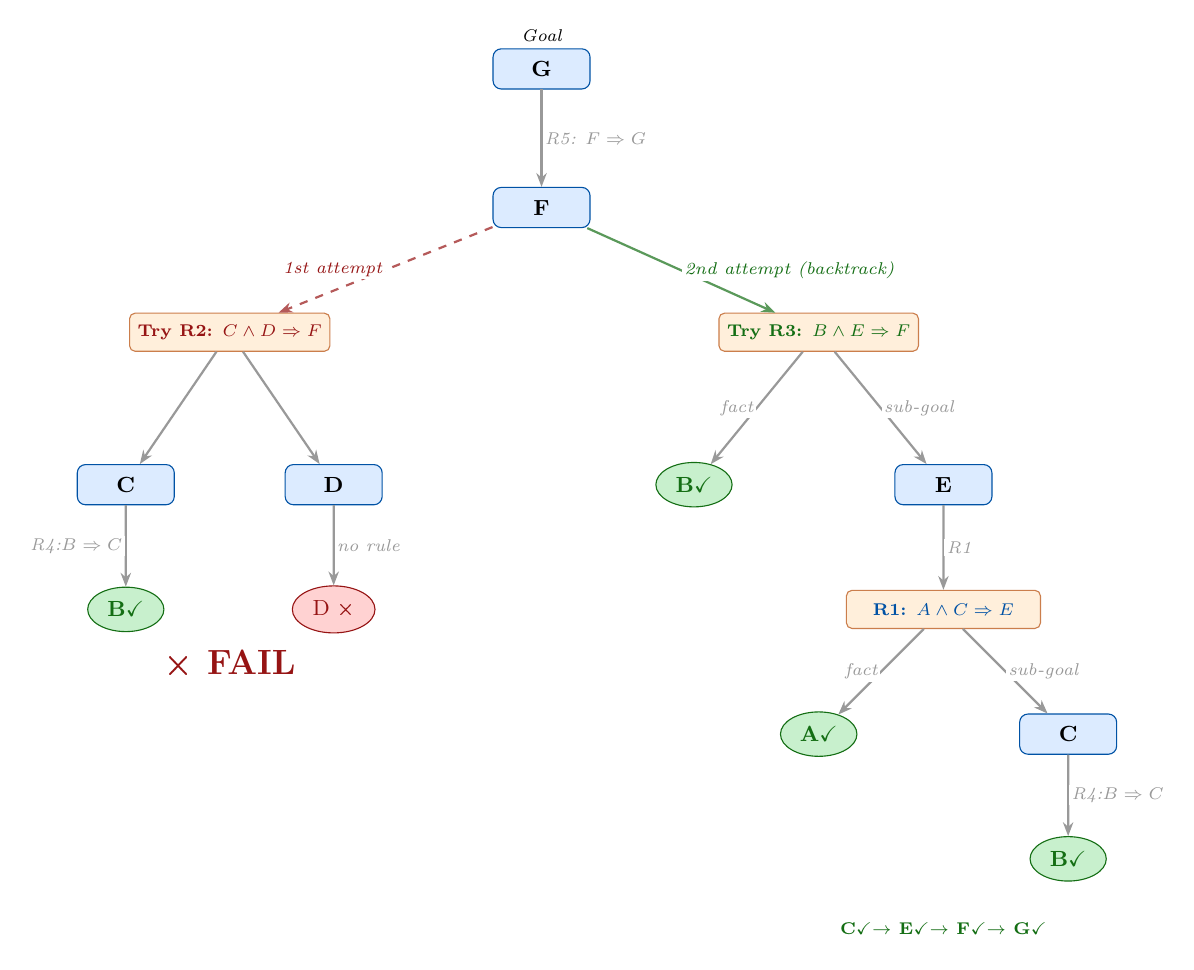
\begin{tikzpicture}[scale=0.88,transform shape]

%% Node styles for this tree
\tikzset{
  BG/.style={rectangle,rounded corners=3pt,draw=ruleblue,fill=lightblue,
             minimum width=1.4cm,minimum height=0.58cm,font=\small\bfseries},
  BP/.style={ellipse,draw=darkgreen,fill=lightgreen,
             minimum width=1.1cm,minimum height=0.52cm,font=\small\bfseries,text=darkgreen},
  BF/.style={ellipse,draw=darkred,fill=lightred,
             minimum width=1.1cm,minimum height=0.52cm,font=\small,text=darkred},
  BRl/.style={rectangle,rounded corners=2pt,draw=darkorange!70,fill=lightorange!80,
              minimum width=2.8cm,minimum height=0.55cm,font=\scriptsize\bfseries},
  ea/.style={arr,gray!80},
  rl/.style={font=\scriptsize\itshape,fill=white,inner sep=1pt},
}

%% Root
\node[BG] (G) at (0,0) {G};
\node[rl,above=0.05cm of G] {\scriptsize Goal};

%% Level 1 via R5
\node[BG] (F) at (0,-2.0) {F};
\draw[ea] (G) -- node[right,rl]{R5: $F\Rightarrow G$} (F);

%% Branch labels
\node[BRl,text=darkred] (R2lbl) at (-4.5,-3.8) {Try R2: $C\wedge D\Rightarrow F$};
\node[BRl,text=darkgreen] (R3lbl) at (4.0,-3.8) {Try R3: $B\wedge E\Rightarrow F$};
\draw[ea,darkred!70,dashed] (F) -- node[left,rl]{\color{darkred}1st attempt} (R2lbl);
\draw[ea,darkgreen!70] (F) -- node[right,rl]{\color{darkgreen}2nd attempt (backtrack)} (R3lbl);

%% R2 branch
\node[BG] (C1) at (-6.0,-6.0) {C};
\node[BG] (D)  at (-3.0,-6.0) {D};
\draw[ea] (R2lbl) -- (C1);
\draw[ea] (R2lbl) -- (D);

\node[BP] (B1) at (-6.0,-7.8) {B\checkmark};
\draw[ea] (C1) -- node[left,rl]{R4:$B\Rightarrow C$} (B1);

\node[BF] (Dfail) at (-3.0,-7.8) {D \texttimes};
\draw[ea] (D) -- node[right,rl]{no rule} (Dfail);

%% Fail cross on R2 branch
\node[font=\Large\bfseries\color{darkred}] at (-4.5,-8.6) {\texttimes\ FAIL};

%% R3 branch
\node[BP] (B2) at (2.2,-6.0) {B\checkmark};
\node[BG] (E)  at (5.8,-6.0) {E};
\draw[ea] (R3lbl) -- node[left,rl]{fact} (B2);
\draw[ea] (R3lbl) -- node[right,rl]{sub-goal} (E);

%% E branch via R1
\node[BRl,text=ruleblue] (R1lbl) at (5.8,-7.8) {R1: $A\wedge C\Rightarrow E$};
\draw[ea] (E) -- node[right,rl]{R1} (R1lbl);

\node[BP] (A2) at (4.0,-9.6) {A\checkmark};
\node[BG] (C2) at (7.6,-9.6) {C};
\draw[ea] (R1lbl) -- node[left,rl]{fact} (A2);
\draw[ea] (R1lbl) -- node[right,rl]{sub-goal} (C2);

\node[BP] (B3) at (7.6,-11.4) {B\checkmark};
\draw[ea] (C2) -- node[right,rl]{R4:$B\Rightarrow C$} (B3);

%% Success annotations
\node[font=\scriptsize\bfseries\color{darkgreen}] at (5.8,-12.4)
  {C\checkmark $\to$ E\checkmark $\to$ F\checkmark $\to$ G\checkmark};

\end{tikzpicture}
\end{center}

\begin{keybox}{Key Observations}
\begin{itemize}
  \item \textbf{Backtracking}: BC tried R2 ($C\wedge D\Rightarrow F$) first. C was proved (via R4 and B),
        but \textbf{D failed} (no rule concludes D; D not in facts). System backtracks to F and tries R3.
  \item \textbf{Goal propagation}: Each goal is either reduced to a known fact or proved via a rule.
  \item \textbf{Sub-goal sharing}: B and C appear in both branches. Real systems use memoization.
\end{itemize}
\end{keybox}

%%==============================================
\section{Expert Systems}
%%==============================================

\begin{defbox}{Definition}
An \textbf{expert system} is a computer program that emulates the decision-making of a
\textbf{human expert} within a specific domain. It applies inference over a domain-specific
knowledge base to solve problems that normally require human expertise.
\end{defbox}

\begin{exambox}{Past Paper}
``What is an expert system? Describe the two essential capabilities.''\\
2021~Q7c [2\,m], 2020~Q7c [2\,m]
\end{exambox}

\subsection{Characteristics}

\begin{itemize}[itemsep=4pt]
  \item Acts in a \textbf{specific domain} and behaves like a human expert within it.
  \item Applied to problems where \textbf{no efficient algorithmic solution exists} ---
        requiring judgment, heuristics, and experiential knowledge.
  \item Guided by \textbf{domain-specific rules} (the knowledge base).
  \item Must be able to \textbf{explain its reasoning}: ``Why did you ask that?''
        and ``How did you reach that conclusion?''
\end{itemize}

\subsection{Two Essential Capabilities}

\begin{enumerate}[itemsep=8pt]
  \item \textbf{Inference Capability (Reasoning and Problem-Solving):}\\
        The system must apply rules and facts to derive new conclusions,
        just as a human expert reasons through a problem.
        This is implemented by the \textbf{inference engine} using FC or BC.
        Without this, the system is merely a static database --- it cannot solve new problems.
        It must handle uncertainty, exceptions, and incomplete data.

  \item \textbf{Explanation Capability (Justification and Transparency):}\\
        The system must explain and justify its conclusions in terms understandable to the user:
        \begin{itemize}
          \item \textbf{``How'' trace:} ``How did you conclude X?'' ---
                shows the chain of rules and facts that produced conclusion X.
          \item \textbf{``Why'' trace:} ``Why are you asking about Y?'' ---
                shows which goal Y is needed to support.
        \end{itemize}
        This transparency distinguishes expert systems from black-box models and
        builds user trust.
\end{enumerate}

\subsection{Notable Expert Systems}

\begin{center}
\renewcommand{\arraystretch}{1.3}
\begin{tabular}{>{\bfseries}p{2.8cm} p{3.2cm} p{7.5cm}}
\toprule
System & Domain & Description \\
\midrule
MYCIN & Medical diagnosis & Diagnosed blood infections; recommended antibiotics (used BC) \\
DENDRAL & Chemistry & Identified molecular structures from mass-spectrometer data \\
R1/XCON & Computer config. & Configured VAX computer systems (DEC) \\
PROSPECTOR & Geology & Assessed mineral deposit likelihood \\
CLIPS & General (FC) & C Language Integrated Production System shell (widely used) \\
NEXPERT & General & Commercial expert system development shell \\
PROLOG & Logic programs & Language with built-in BC; basis for many ES \\
\bottomrule
\end{tabular}
\end{center}

%%==============================================
\section{Frames (Structured Knowledge Representation)}
%%==============================================

\begin{defbox}{Definition}
A \textbf{frame} is a data structure for representing a stereotyped concept or object.
It consists of a set of \textbf{slots} (attributes), each holding a value.
A frame captures the ``prototype'' of a concept; an \textbf{instance} of a frame
represents a specific individual object of that concept.
\end{defbox}

\subsection{Structure}

\begin{center}
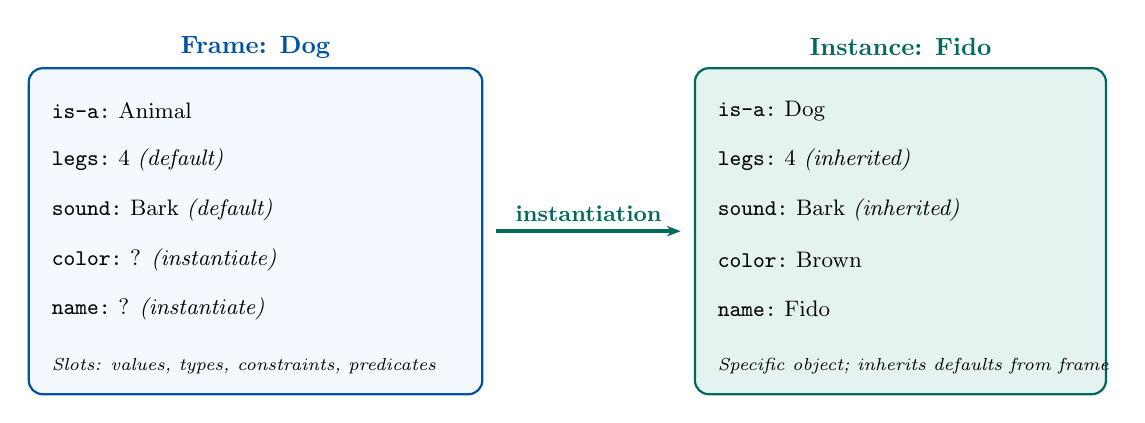
\begin{tikzpicture}[scale=0.9,transform shape]
%% Frame: Dog
\draw[rounded corners=5pt,draw=ruleblue,fill=lightblue!30,thick]
  (-3.2,0) rectangle (3.2,-4.6);
\node[font=\bfseries\color{ruleblue}] at (0,0.3) {\textsc{Frame: Dog}};
\node[font=\small,anchor=west] at (-3.0,-0.6) {\texttt{is-a:}\ Animal};
\node[font=\small,anchor=west] at (-3.0,-1.3) {\texttt{legs:}\ 4 \textit{(default)}};
\node[font=\small,anchor=west] at (-3.0,-2.0) {\texttt{sound:}\ Bark \textit{(default)}};
\node[font=\small,anchor=west] at (-3.0,-2.7) {\texttt{color:}\ ? \textit{(instantiate)}};
\node[font=\small,anchor=west] at (-3.0,-3.4) {\texttt{name:}\ ? \textit{(instantiate)}};
\node[font=\scriptsize\itshape,anchor=west] at (-3.0,-4.2) {Slots: values, types, constraints, predicates};

%% Arrow
\draw[arr,darkteal,line width=1.5pt] (3.4,-2.3) --
  node[above,font=\small\bfseries,text=darkteal]{instantiation} (6.0,-2.3);

%% Instance: Fido
\draw[rounded corners=5pt,draw=darkteal,fill=lightteal!50,thick]
  (6.2,0) rectangle (12.0,-4.6);
\node[font=\bfseries\color{darkteal}] at (9.1,0.3) {\textsc{Instance: Fido}};
\node[font=\small,anchor=west] at (6.4,-0.6) {\texttt{is-a:}\ Dog};
\node[font=\small,anchor=west] at (6.4,-1.3) {\texttt{legs:}\ 4 \textit{(inherited)}};
\node[font=\small,anchor=west] at (6.4,-2.0) {\texttt{sound:}\ Bark \textit{(inherited)}};
\node[font=\small,anchor=west] at (6.4,-2.7) {\texttt{color:}\ Brown};
\node[font=\small,anchor=west] at (6.4,-3.4) {\texttt{name:}\ Fido};
\node[font=\scriptsize\itshape,anchor=west] at (6.4,-4.2) {Specific object; inherits defaults from frame};
\end{tikzpicture}
\end{center}

\subsection{Slot Contents}

Each slot can contain:
\textbf{Values} (actual data), \textbf{Types} (expected data type),
\textbf{Constraints} (valid value ranges), \textbf{Predicates} (logical conditions),
\textbf{Pointers} to other frames (nested structures).

Frames are analogous to \textbf{OOP classes}: frame $\approx$ class, instance $\approx$ object,
slot $\approx$ attribute.

\subsection{Inferencing with Frames}

\begin{enumerate}[itemsep=4pt]
  \item \textbf{Default values:} If a slot is unfilled in an instance, the frame's default applies.
        Reduces redundancy.
  \item \textbf{Generic values:} Class-level values inherited by all instances.
  \item \textbf{Inheritance:} Instances inherit slot values from their frame.
        \textbf{Multiple inheritance} allows a frame to inherit from multiple parents.
\end{enumerate}

%%==============================================
\section{Exam Strategy Summary}
%%==============================================

\subsection{Q6 Template (Appears Every Year)}

\begin{center}
\renewcommand{\arraystretch}{1.4}
\begin{tabular}{c p{8.5cm} r}
\toprule
\textbf{Part} & \textbf{Required Content} & \textbf{Marks} \\
\midrule
Q6(a) & Define FC + BC. State 4 factors for choosing between them. & $\sim$2 \\
Q6(b) & Define conflict resolution. Explain any 2 strategies. & $\sim$1.5 \\
Q6(c) & Draw RBS architecture diagram. Prove G via FC (trace table + tree).
        Prove G via BC (trace table + tree with backtracking). & $\sim$6 \\
\midrule
\multicolumn{2}{r}{\textbf{Total for this question}} & \textbf{$\approx$9--10} \\
\bottomrule
\end{tabular}
\end{center}

\subsection{Past Paper Coverage (2020--2024)}

\begin{center}
\renewcommand{\arraystretch}{1.3}
\begin{tabular}{p{6.5cm} ccccc}
\toprule
\textbf{Topic} & \textbf{2024} & \textbf{2023} & \textbf{2022} & \textbf{2021} & \textbf{2020} \\
\midrule
RBS Architecture & Q6c & Q6c & B3 & Q5c & Q5c \\
FC definition + factors & Q6a & Q6a & B3b & Q5a & Q5a \\
BC definition + factors & Q6a & Q6a & B3b & Q5a & Q5a \\
Conflict resolution + 2 strategies & Q6b & Q6b & B3a & Q5b & Q5b \\
FC proof: R1--R5 $\Rightarrow$ G & Q6c & Q6c & B3c & Q5c & Q5c \\
BC proof: R1--R5 $\Rightarrow$ G & Q6c & Q6c & B3c & Q5c & Q5c \\
Expert system + 2 capabilities & --- & --- & --- & Q7c & Q7c \\
\bottomrule
\end{tabular}
\end{center}

\begin{keybox}{5 Things to Memorize Cold}
\begin{enumerate}
  \item \textbf{Architecture}: 5 components --- Rule Base, Fact Base, Working Memory,
        Inference Engine (Match-Resolve-Act), User Interface / Explanation Facility.
  \item \textbf{FC firing sequence}: R4 $\to$ R1 $\to$ R3 $\to$ R5.
        WM grows: $\{A,B\}\to\{A,B,C\}\to\{A,B,C,E\}\to\{A,B,C,E,F\}\to\{A,B,C,E,F,G\}$.
  \item \textbf{BC proof chain}: $G\leftarrow F\leftarrow(B_\checkmark, E\leftarrow(A_\checkmark, C\leftarrow B_\checkmark))$.
        Key: R2 fails on D; backtrack to R3.
  \item \textbf{FC vs BC}: 4 factors --- data availability, goal specificity,
        branching factor, data acquisition cost.
  \item \textbf{Conflict resolution}: 2 best to explain --- Rule Ordering (FCFS) +
        Specificity Ordering. Add Refractoriness as a bonus.
\end{enumerate}
\end{keybox}

\end{document}
